
\subsection{%Микроархитектура %процессора 
Структура
Intel 8008
и~Core2}

\begin{tabularx}{1\linewidth}{@{}l@{\,}l@{}}
% 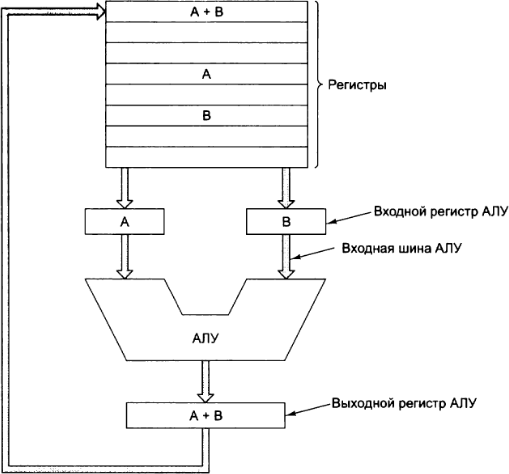
\includegraphics[width=0.7\linewidth,valign=c]{data-path}


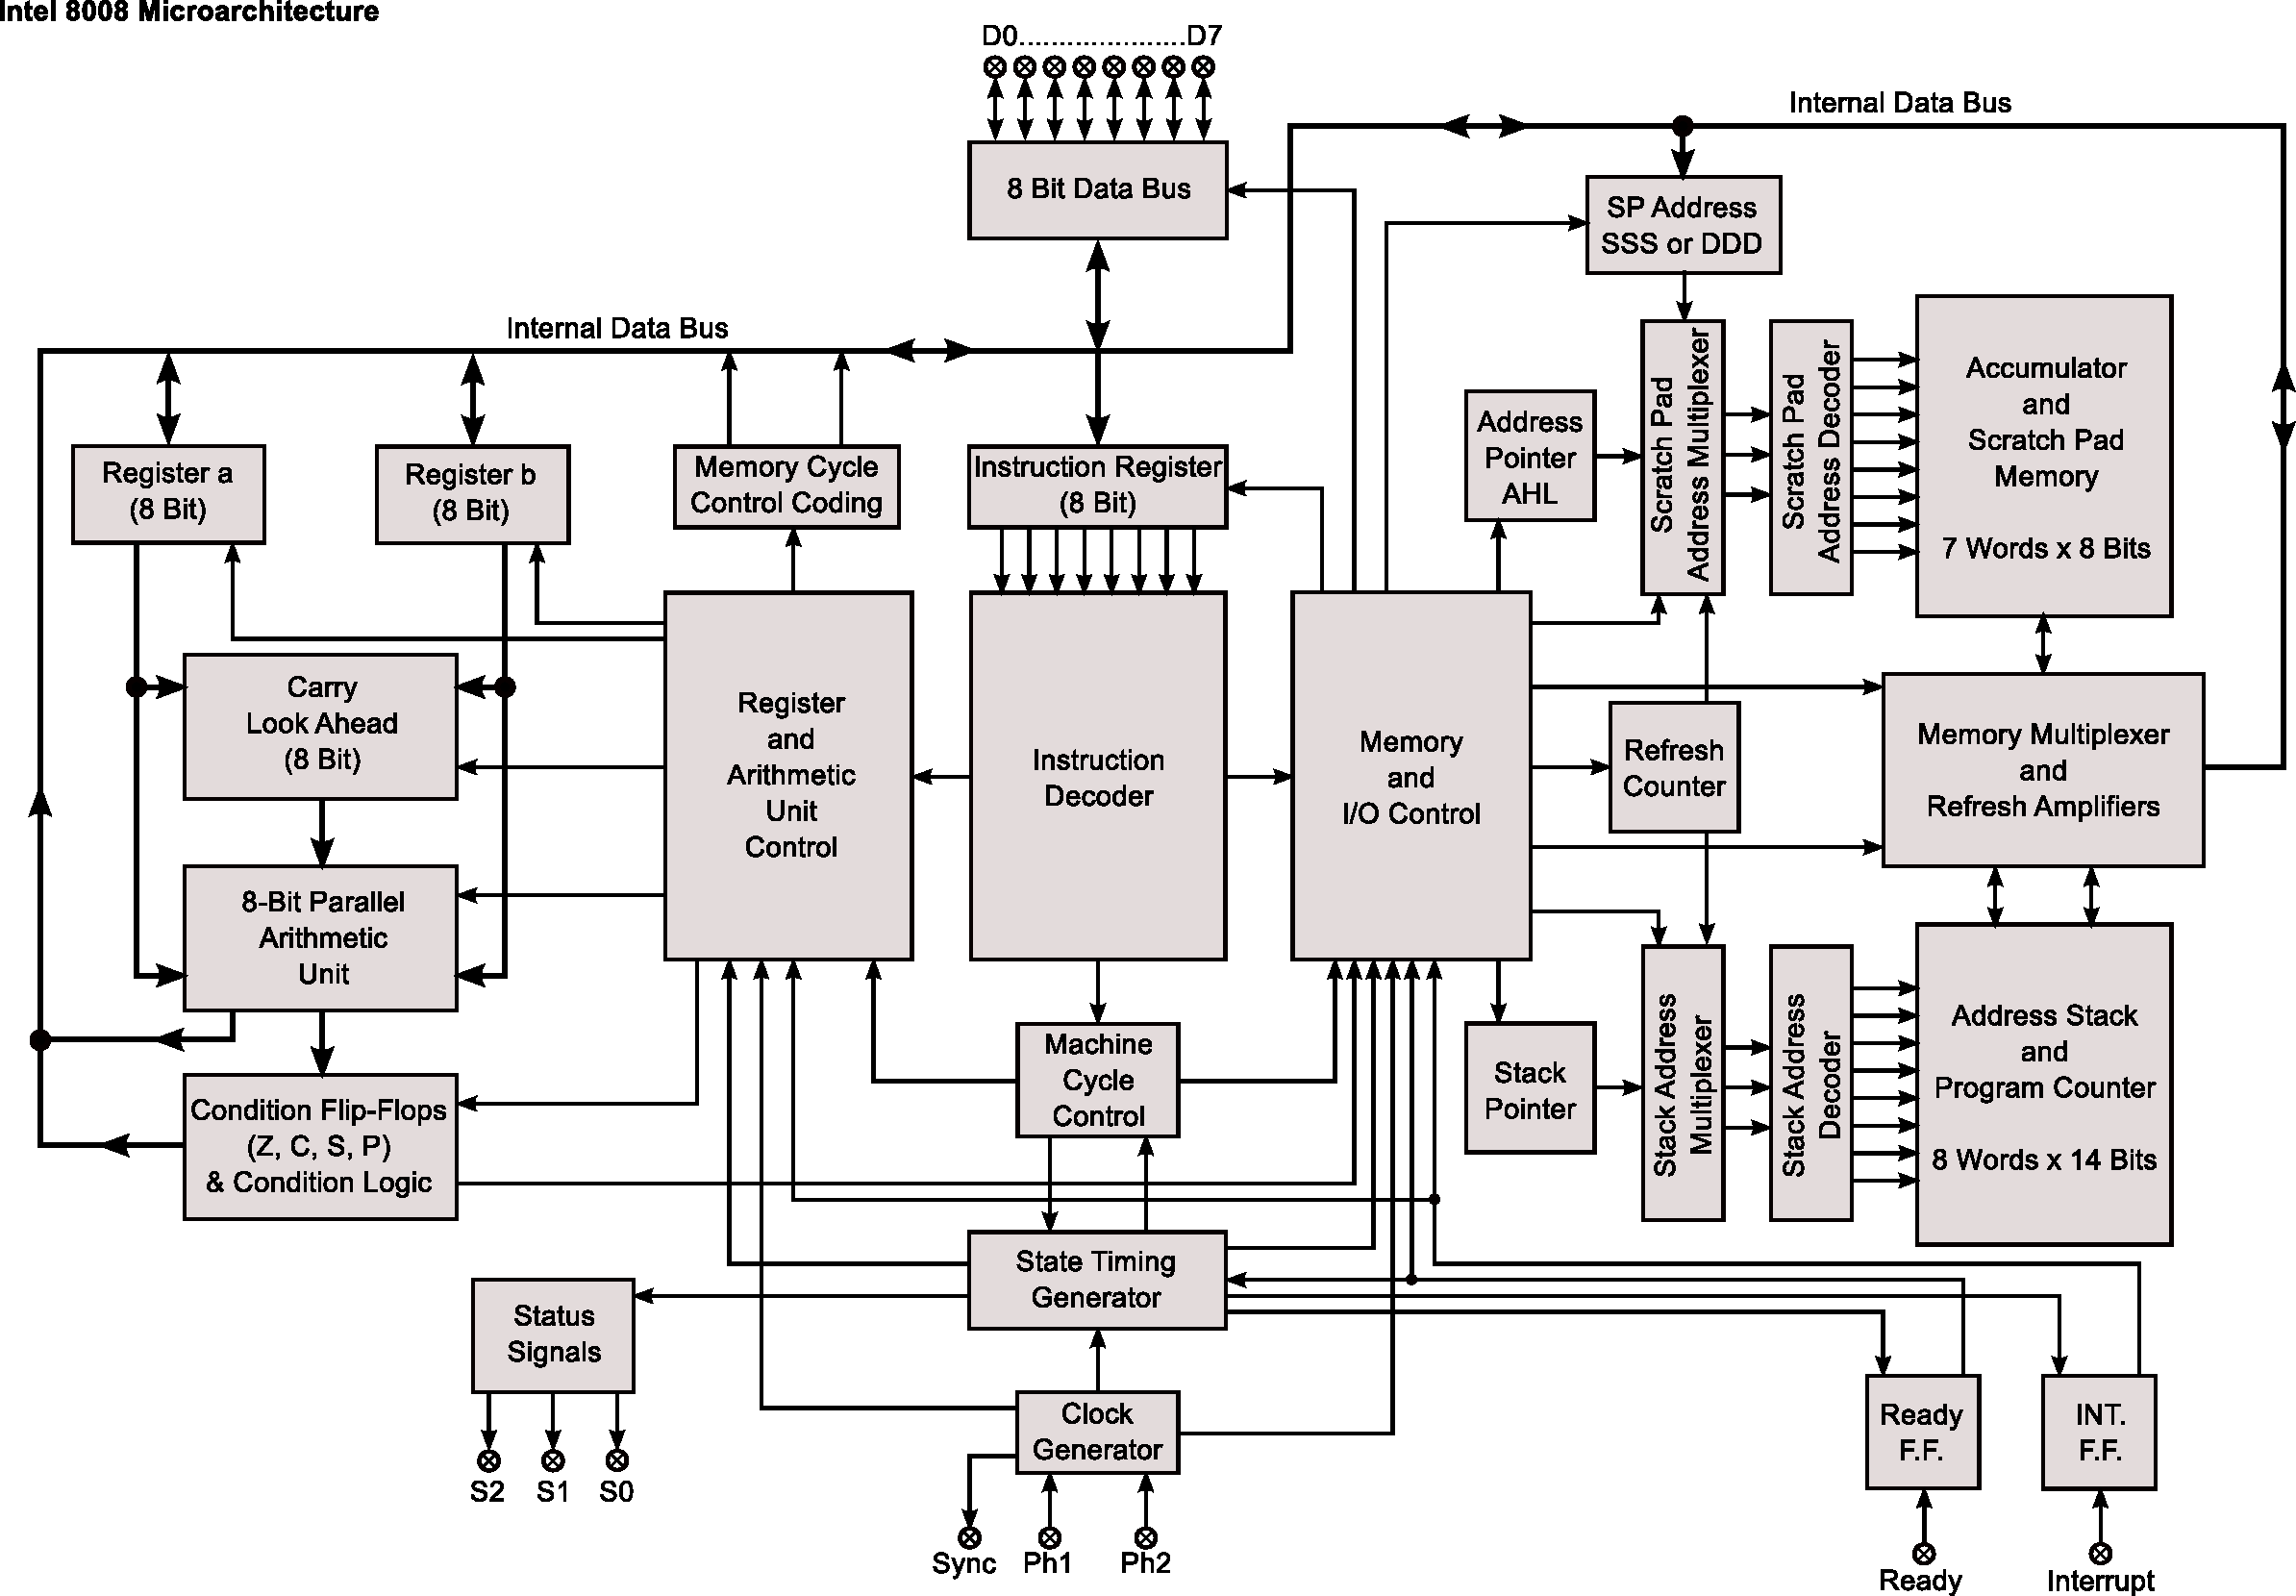
\includegraphics[width=0.595\linewidth,keepaspectratio,valign=c]{Intel_8008_arch}\centering
&

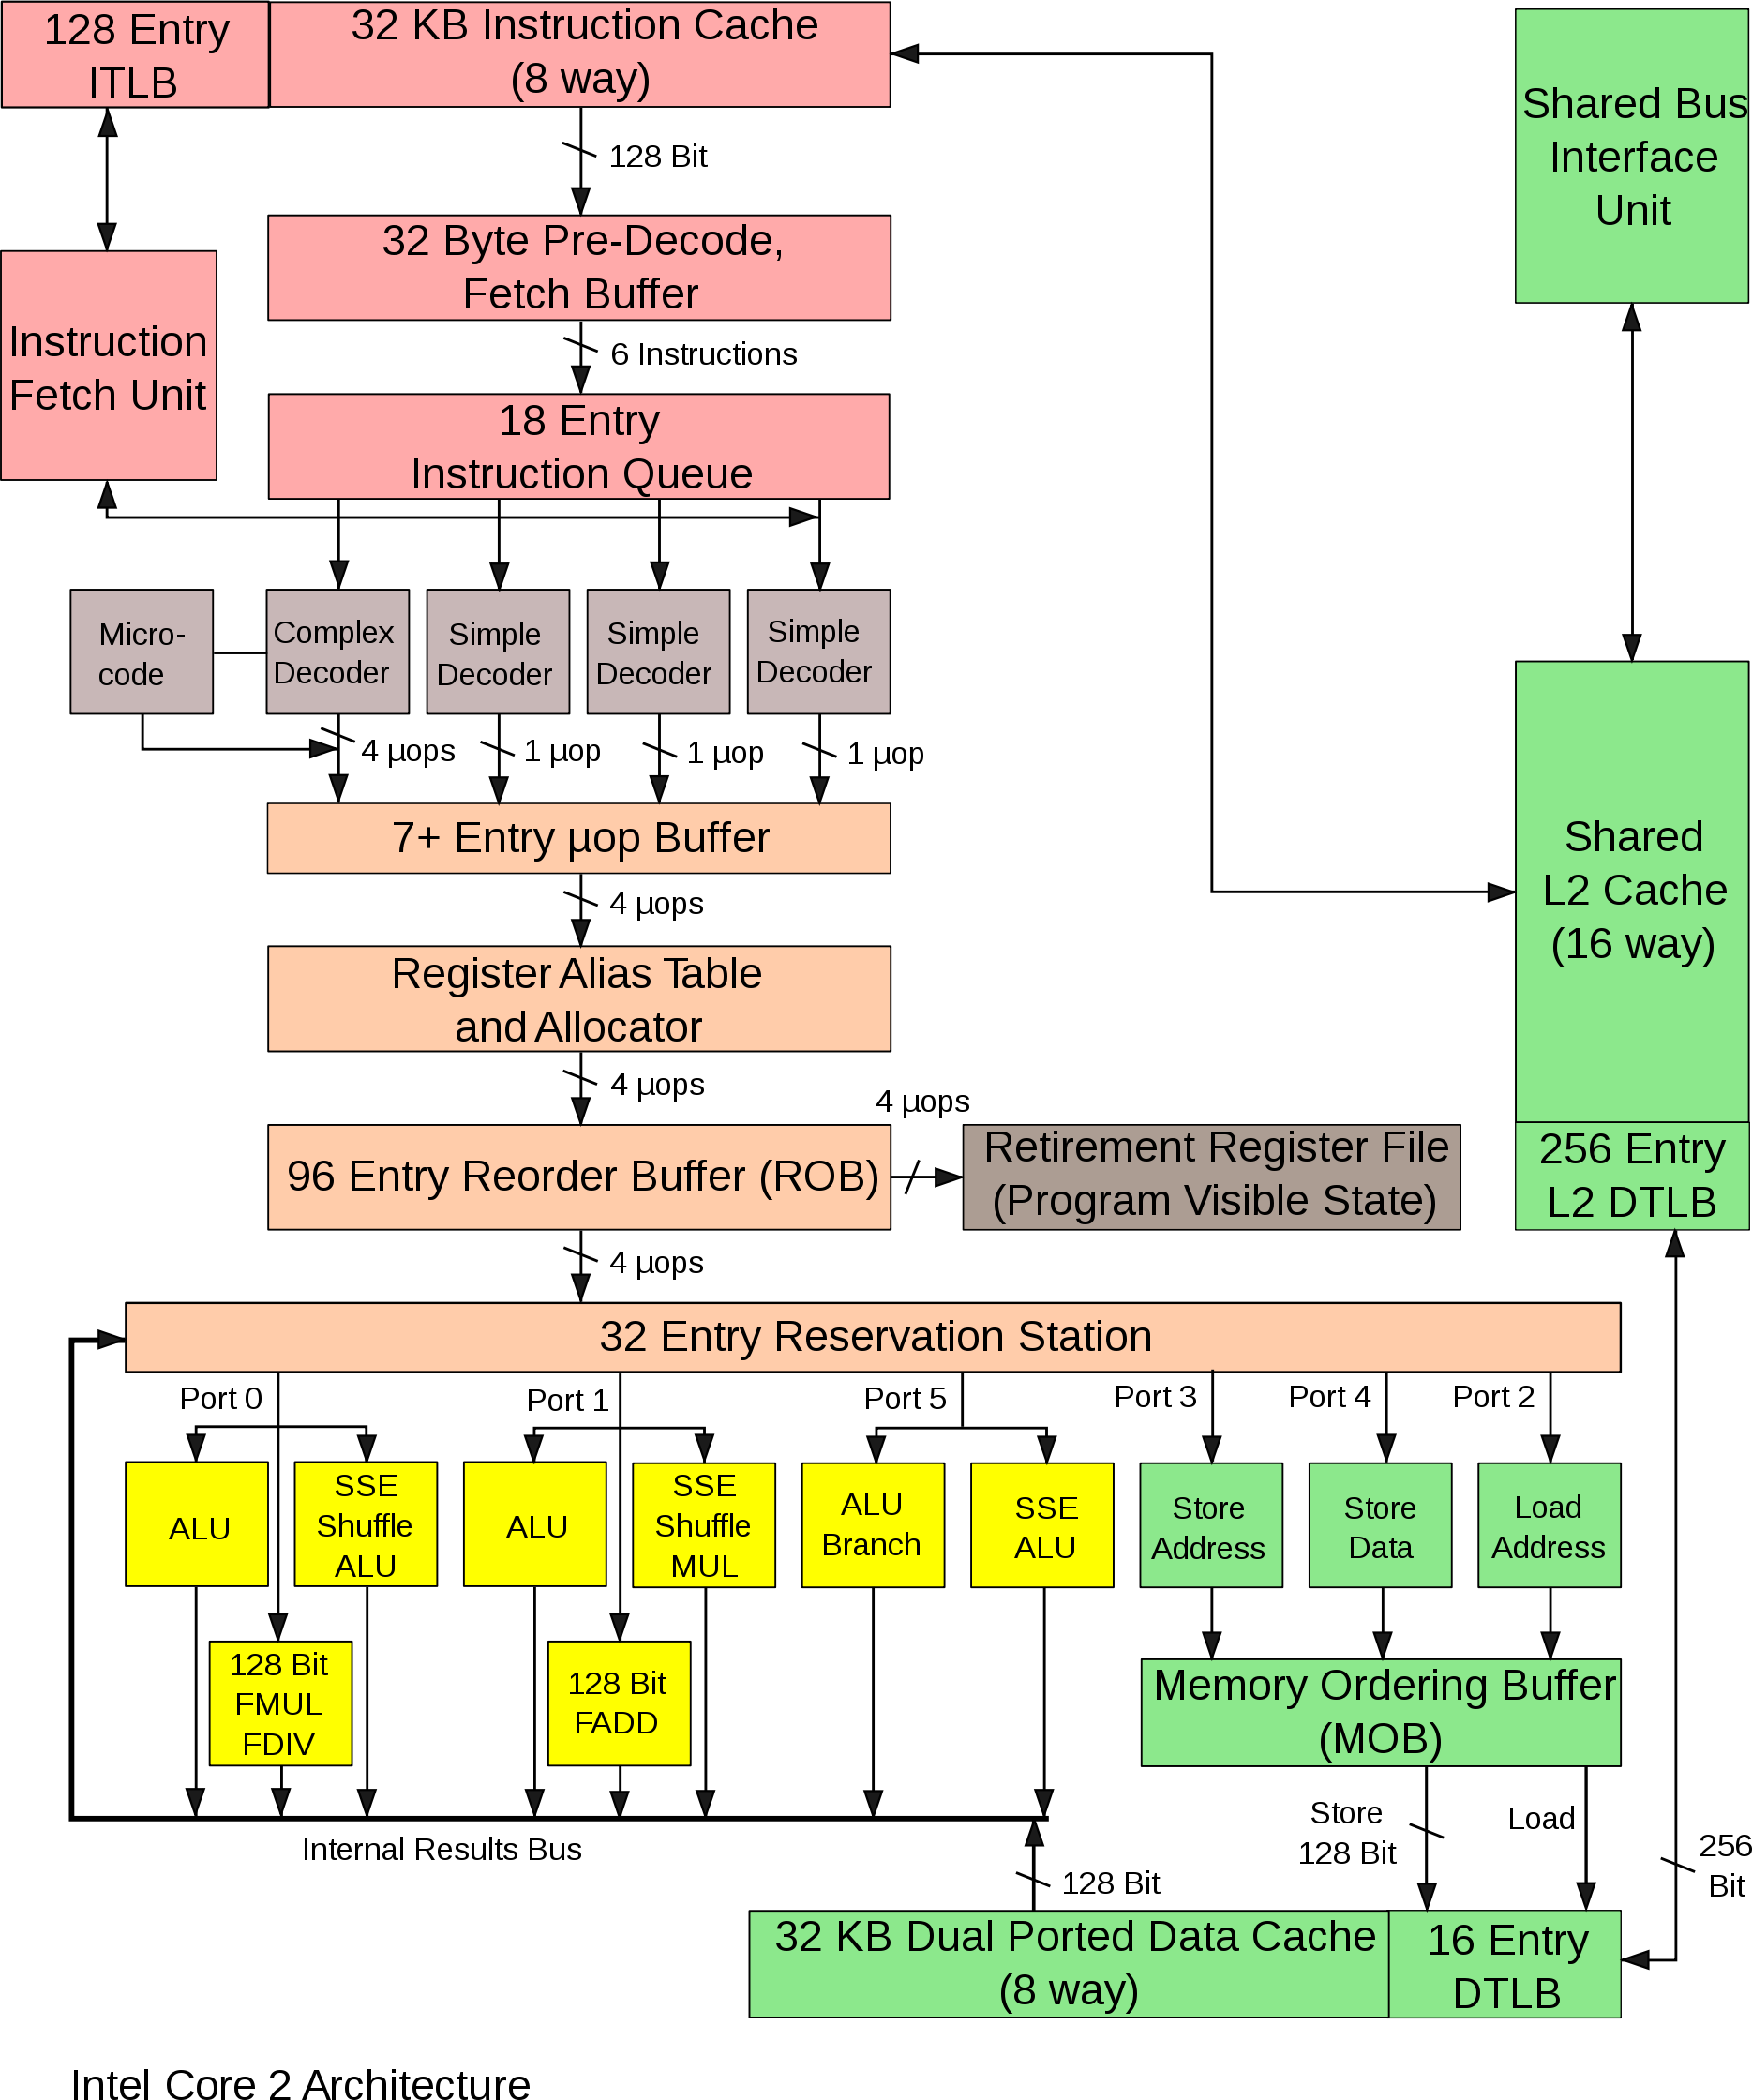
\includegraphics[width=0.395\linewidth,keepaspectratio,valign=c]{Intel_Core2_arch}
\end{tabularx}



\subsection{Магистрали}
% \subsection{Макроархитектура}
% \subsection{Функциональная схема компьютера}
% \begin{frame}{\insertsubsection}
% \footnotesize
% {
% 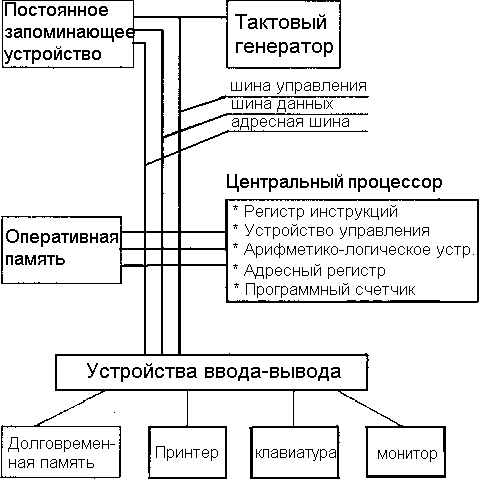
\includegraphics[height=\slideheigth,valign=t]{func-comp}\centering
% 
% }
% 
% \end{frame}


\resizebox{0.8\linewidth}{!}{
\newlength{\ndist}
\setlength{\ndist}{2ex}

% \tikzstyle{blockarrow}	= [-latex',thick,draw]
\begin{tikzpicture}[
start chain=uvv going right,
start chain=bus_south going right,
% start chain=bus_north going below,
start chain=bus_comment going above,
start chain=bus_vdown going below,
start chain=bus_vup going above,
% every on chain/.style=join,
% every on chain/.style=solidchaincell,
% every join/.style=blockarrow,
node distance=\ndist and 2ex,
baseline=(current bounding box.north)
]
\tikzstyle{strokednode}	= [text badly centered, draw=black, thick, inner xsep = \ndist]
\tikzstyle{block}	= [strokednode, text width=18ex, minimum height=6ex]


% \tikzstyle{bus}	= [ultra thick, draw=black!80!green]
\tikzstyle{bus}	= [very thick,double]
% \tikzstyle{powerline}	= [draw=green]
\tikzstyle{powerline}	= []
% \tikzstyle{buscommentstyle}	= [blue,thin, text=blue]
\tikzstyle{buscommentstyle}	= [densely dashed,thin]


\node[block, on chain=uvv] (hdd) {�������������� ������};
\node[block, on chain=uvv] (prn) {�������};
\node[block, on chain=uvv] (kbd) {����������};
\node[block, on chain=uvv] (mon)  {�������};
\node[fit=(hdd) (mon), inner sep=0ex] (uvv_box) {};

\node[block, text width=42ex, above=2\ndist of uvv_box] (uvv_common) {���������� �����-������};

\foreach \i in {hdd, prn, kbd, mon}
{
  \draw[] (\i.north) -- (uvv_common);
}

\coordinate[left = 0.5\ndist of uvv_common.north] (centerleftbus_south);

\coordinate[on chain=bus_south, left = of centerleftbus_south] (addr_south);
\coordinate[on chain=bus_south] (data_south);
\coordinate[on chain=bus_south] (ctrl_south);
\coordinate[on chain=bus_south] (power_south);

\coordinate[right = 2\ndist of power_south] (rightblocks_west);

\tikzstyle{block}	= [strokednode, text width=18ex, minimum height=10ex]

% \node[strokednode, text width=33ex, text badly ragged, above right = 2\ndist of power_south] (cpu)  {
\node[strokednode, text width=27ex, text badly ragged, above  = 2\ndist of rightblocks_west, anchor=south west] (cpu)  {
����������� ���������
% \setlength{\leftmargini}{14ex}
\begin{itemize}[leftmargin=*,topsep=0pt,itemsep=0pt]
\item ���;
% \item ���������� ����������;
\item ��;
\item �������� ���.
% % \item �������� �������; 
% \item ������� ������; 
% \item ��������� �������.
\end{itemize}
};

\tikzstyle{highest} = [above = 1.5\ndist of cpu.west]
\foreach \i/\pos in {addr/highest, data/, ctrl/, power/}
{
  \coordinate[on chain=bus_vdown, \pos] (\i_cpu);
}

\node[block, left = 2\ndist of addr_south|-cpu.west] (ram)  {����������� ������};



\foreach \i/\s in {addr/, data/, ctrl/, power/powerline}
{
  \draw[bus, \s] (ram.east|-\i_cpu) -- (cpu.west|-\i_cpu);
}

{

  \tikzset{node distance=3ex}
  % \tikzset{buscommentstyle}

  \coordinate[above =  of cpu.north-|addr_south, on chain=bus_comment] (addr_comment);
  \coordinate[on chain=bus_comment] (data_comment);
  \coordinate[on chain=bus_comment] (ctrl_comment);
  \coordinate[on chain=bus_comment] (power_comment);

  \coordinate (end_comment) at (cpu.east);


  \foreach \i/\s in {addr/������, data/������, ctrl/����������, power/\vphantom{�}�������}
  {
    \draw[buscommentstyle](\i_comment-|\i_south) -- node[above=-1ex, buscommentstyle, at end, anchor=south east, text badly ragged] {���� \s} (\i_comment-|end_comment);
  }
}


% \node[block, above = 16ex of ram] (bios)  {���������� ������������ ����������};
% \node[block, right =4ex of bios-|power_south] (clock)  {�������� ���������};

\node[block, above = 2\ndist of power_comment-|rightblocks_west, anchor=south west] (clock)  {�������� ���������};
\node[block, left = 2\ndist of addr_south|-clock] (bios)  {���������� ������������ ����������};


% \coordinate[above = of bios.east-|ctrl_south] (ctrl_north);
% \coordinate (data_north) at (bios.east);
% \coordinate[below = of data_north] (addr_north);
% 
% \coordinate[above = of ctrl_north-|power_south] (power_north);

% \tikzstyle{highest} = [above = 1.5\ndist of bios.east]
% \foreach \i/\pos in {addr/highest, data/, ctrl/, power/}
% {
%   \coordinate[on chain=bus_vdown, \pos] (\i_vnorth);
%   \coordinate (\i_north) at (\i_vnorth-|\i_south);
% }
\tikzstyle{lowest} = [below = 1.5\ndist of bios.east]
\foreach \i/\pos in {addr/lowest, data/, ctrl/, power/}
{
  \coordinate[on chain=bus_vup, \pos] (\i_vnorth);
  \coordinate (\i_north) at (\i_vnorth-|\i_south);
}

\foreach \i/\s in {ctrl/, power/powerline}
{
  \draw[bus, \s] (\i_south) -- (\i_north);
  \draw[bus, \s] (bios.east|-\i_north) -- (clock.west|-\i_north);
}

% \draw[bus] (data_south) |- (data_north);
% \draw[bus] (addr_south) |- (addr_north);

\foreach \i/\s in {addr/, data/}
{
  \draw[bus] (\i_south) -- (\i_north) -- (\i_vnorth);
}

% \draw (bios) -- coordinate () (clock);

\end{tikzpicture}
}
